\section{Key Results}
Dieser Abschnitt beschäftigt sich mit unserer Umsetzung der Aufgaben des Meta-Bereichs. Unser Ziel war es, nach jedem Durchlauf zu "lernen", indem man das vorherige Handeln speichert, evaluiert und dies beim wiederholten Durchlauf berücksichtigt.

\subsection{Level und Datenbank}

\subsubsection{Level}
Zur Speicherung der ausgeführten Aktionen wird eine Datenbank benötigt. Doch bevor man solch eine für die verschiedenen Level bauen kann, müssen die grundlegenden Informationen kompatibel sein: das Level selber. Unsere Java-Klasse \texttt{Level} befindet sich im Ordner \texttt{Meta}. Diese besteht aus der Level-ID, den geschätzten maximal zu erreichenden Punkten dieses Levels, den tatsächlich erreichten Punkten, der Anzahl der gespielten Durchgänge und einer Liste von ausgeführten Schüssen. Das Zusammenfassen der Schüsse erfolgt durch die selber errichtete Klasse \texttt{Triplet}, die sich auch im \texttt{Meta}-Ordner befindet. Hierbei wird neben dem eigentlichen Schuss (\texttt{shot}) zusätzlich noch das anvisierte Zielobjekt (\texttt{target}) und die allein aus diesem Schuss erreichten Punkte (\texttt{damagePoints}) gespeichert, welche später in der \texttt{ShotSelection} relevant sind. \\
Die Klasse an sich dient als Grundlage und enthält dementsprechend nur wenige Methoden, wobei einige bereits von der Gruppe aus dem letzten Jahr geschrieben wurden und wir nur noch unsere Änderungen anpassen mussten (siehe \texttt{addExecutedShot}) bzw. die Methoden verbessert haben (siehe \texttt{calculateEstimatedMaximalPoints}). 

\subsubsection{Datenbank}
Nach jedem Durchlauf eines Levels werden die oben genannten Informationen in ein \texttt{Level}-Objekt gespeichert. Jedes einzelne \texttt{Level}-Objekt wird dann in eine Datenbank hinzugefügt, welche unter \menu{ database > LevelStorage} zu finden ist. \\
Der Ordner \texttt{database} enthält eine weitere enum-Klasse \texttt{LevelState}, welche nur der Markierung der Level dient, weiter aber noch keine Verwendung findet. \\ 
Die \texttt{LevelStorage} besteht aus einer privaten Map, die die \texttt{Level} und den dazugehörigen \texttt{LevelState} beinhaltet. Zusätzlich enthält die Klasse eine öffentlichen Liste aus Integer, die in der gleichen Reihenfolge wie der Map die Level-IDs der gespielten Level speichert, sodass man von außen schnell auf die Information zugreifen kann, welche Level bereits gespielt wurden, sowie den Index der Level leichter abfragen kann. \\
Beim Speichern der Level muss darauf geachtet werden, dass man die Level nicht doppelt speichert im Falle eines wiederholten Versuchs. Daher prüfen wir in unserer öffentlichen Methode \texttt{addLeveltoStorage}, ob das übergebene Level bereits in der Datenbank erhalten ist. Falls es einen Eintrag mit dieser Level-ID gibt, wird die Hilfsmethode \texttt{updateLevelInfo} aufgerufen, welche nur die geänderten Einträge aktualisiert, anstatt einen komplett neuen Eintrag zu erstellen. \\
Die \texttt{LevelStorage} ist in der Evaluation von großer Bedeutung und wird in den Klassen der nachfolgenden Kapitel verwendet.

\subsection{Level Selection}
Die Klasse \texttt{LevelSelection}, die sich im Ordner \texttt{Meta} befindet, ist für die Levelauswahl zuständig. Sie hält die Information über die gesamte Anzahl der zu spielenden Level und über das Level, das gerade gespielt wird. Die Hauptmethode \texttt{selectNextLevel} beginnt mit einer zufällig ausgewählten Levelnummer und geht beim ersten Durchlauf alle Level der Reihenfolge nach durch. \\
Sobald alle Level einmal durchgespielt wurden, muss nun entschieden werden, welche Level in welcher Reihenfolge und wie oft wiederholt werden sollen. \\
Die Auswahl erfolgt nach einer simplen Wahrscheinlichkeitsberechnung für jedes einzelne Level, wobei das Level mit der höchsten Wahrscheinlichkeit ausgewählt wird: \\
$$ Probability = 1 - ( actualScore / maximalReachableScore ) $$
Wir richten uns also danach, wie viele Punkte wir von der maximal möglichen Punktzahl bereits abdecken konnten. \\
Eine Besonderheit gibt es für verlorene Level, welche als erste ausgewählt werden, denn ihre tatsächlich erbrachte Punktzahl beträgt 0 und sie haben somit eine Wahrscheinlichkeit von 1. Da man für jedes Level im Durchschnitt mindestens drei Minuten erhält \footnote{https://aibirds.org/angry-birds-ai-competition/competition-rules.html (zuletzt abgerufen: 05.09.2017)} und wir von einer Durchschnittsspieldauer von 1 - 1,5 Minuten pro Level ausgingen, entschieden wir uns, die verlorenen Level zunächst höchstens zweimal wiederholen zu lassen. Falls die Quote der verlorenen Level im Bezug auf die Gesamtanzahl der zu spielenden Level dann immer noch zu hoch ist, soll der Agent ein weiteres verlorenes Level auswählen. In unserem Fall haben wir die Grenze auf 15\% gesetzt, d.h. der Agent würde bei einer Gesamtanzahl von 21 Level einen erneuten Versuch starten, wenn mehr als 3 Level noch verloren sind. Falls dann immer noch nicht alle Level gewonnen wurden, sollen diese ignoriert werden. \\ 
Zur Veranschaulichung, wie der Algorithmus implementiert werden soll, dient der Pseudocode \ref{lvlSelec}. Hierbei haben wir einen boolean-Wert \texttt{ignoreLostLevels} integriert, der erst dann auf \textbf{true} gesetzt wird, wenn alle verlorenen Level zweimal wiederholt wurden und die Quote der verlorenen Level unter 15\% beträgt. Dieser Wert wird dann in der zweiten if-Schleife geprüft. \\
\begin{algorithm}[H]
  \begin{algorithmic}[1]
  	\State \textbf{boolean} \textit{ignoreLostLevels} = false
  	\\
  	\State \funccall{calculateProbabilities}() \Comment{calculates the probability for every level}
  	\\
  	\If{lost levels exist}
  		\If{all lost levels were repeated twice}
  		 	\If{Amount of lost levels > 15\% of total number of levels} 
  		 		\hspace{\algorithmicindent}  \Return \funccall{next lost level} \Comment{redo the lost levels one more time}
			\Else  
				\State \textit{ignoreLostLevels} = true
  		 	\EndIf
  		\Else
  			\Return \funccall{next lost level that has not been played twice yet}
  		\EndIf
  	\EndIf
  	\\
  	\If{no lost levels exist \textbf{or} \textit{ignoreLostLevels} == true}
		\Return level with the highest probability  	
  	\EndIf
  \end{algorithmic}
  \caption{Level selection after every level was played at least once \label{lvlSelec}}
\end{algorithm}

\subsection{Shot Selection}
Um bei wiederholten Versuchen von Level nicht ständig dieselben Schüsse zu nehmen und unsere Spieltaktik zu verbessern, kommt nun die Schussauswahl ins Spiel. Dafür bekommt unsere Klasse \texttt{ShotSelection}, die sich ebenfalls im \texttt{Meta}-Ordner befindet, von der Strategie-Gruppe für jeden Vogel eine Liste von Zielobjekten (\texttt{Targets}), auf die der Vogel schießen soll (siehe Methode \texttt{chooseShotWithOneList}). Eines davon wandeln wir dann in ein \texttt{Shot}-Objekt um und der Agent kann den Schuss dann im Spiel ausführen. Nachdem ein Schuss getätigt wurde, wird dieser dann für das entsprechende Level in eine Liste von Schüssen gespeichert (siehe Kapitel \textit{4.1.1 Level}).\\
Zu den jeweiligen \texttt{Targets} wird eine Konfidenz zwischen 0 und 1 mitübergeben, nach welcher der auszuführenden Schuss ausgewählt wird. 

\subsubsection{Verhindern von Wiederholen von Schüssen}
Hierbei besteht die Gefahr, dass immer derselbe Schuss genommen wird. Dies kann eintreten, wenn ein Schuss einer hohen Konfidenz zugeordnet wird, im echten Spiel jedoch wenig oder sogar keine Wirkung auf die Schweine und Gebäude hat. Da nach jedem Schuss neue Pläne in Bezug auf den jetzigen Stand der Umgebung generiert werden und sich die Szene nicht verändert, erhalten wir von der Strategie-Gruppe stets die gleiche Liste von Plänen. Würden wir also den Algorithmus ohne Einschränkung lassen, würde immer das Zielobjekt mit der höchsten Konfidenz ausgewählt werden, welches bei gleichen Szenen immer denselben Schuss entspricht. 
Somit haben wir einen Algorithmus integriert, der in Bezug auf die noch übrig gebliebenen Vögel entscheidet, ob der Schuss ein zweites Mal probiert werden soll, da es auch oft der Fall ist, dass der erste Schuss die Gebäude zum Wackeln gebracht hat und ein zweiter Schuss auf das gleiche Ziel ein guter Zug wäre. Dies lassen wir jedoch nur zu, wenn die Chance noch hoch genug ist, mit den restlichen Vögeln das Level trotz eines zweiten Fehlschusses noch gewinnen zu können. Dies wird in folgendem Pseudocode \ref{ShotSelec} veranschaulicht, wo wir uns nach des Gesamtzahl der Vögel richten: \\
\begin{algorithm}[H]
  \begin{algorithmic}[1]
  \If{shotCandidate.equals(previousShot)}
  	\If{(totalBirdAmount <= 3 \&\& executedShots >= 2) \textbf{or} \\ 
  	\hspace{\algorithmicindent} (totalBirdAmount > 3 \&\& previousPreviousShot.equals(previousShot))}
  	\\ \hspace{2.5em} \funccall{choose another shotCandidate}
  	\Else \\
  		\hspace{2.5em} \funccall{proceed with the current shotCandidate}
  	\EndIf
  \EndIf
  \end{algorithmic}
  \caption{Prevention of endless repetition in ShotSelection \label{ShotSelec}}
\end{algorithm}

\begin{table}[H]
\begin{itemize}
\item \textit{shotCandidate}: der zu prüfende Schuss, der ausgeführt werden soll 
\item \textit{previousShot}: der Schuss, der als letztes tatsächlich ausgeführt wurde
\item \textit{previousPreviousShot}: der Schuss, der vor dem zuletzt ausgeführten Schuss ausgeführt wurde
\end{itemize}
\end{table}

In unserem Algorithmus wird also nur derselbe Schuss noch einmal ausgeführt, wenn die Gesamtanzahl der Vögel über 3 beträgt und die zwei Schüsse davor nicht schon dieselben Schüsse waren, d.h. ein Schuss darf nicht mehr als einmal wiederholt werden. Im Falle von höchstens drei Vögel, wird ein anderer Schuss ausgewählt, wenn es sich gerade um den letzten Schuss handelt.

\subsubsection{Schussevaluation}
Falls das Level bereits gespielt wurde, überprüfen wir zunächst, ob der ausgewählte Schuss beim letzten Durchgang ebenfalls schon an dieser Stelle zum Einsatz kam und ob er ``gut'' oder ``schlecht'' war. Dementsprechend soll ein anderes Zielobjekt ausgewählt werden, wenn der Schuss als \textbf{BAD} markiert wurde. \\
Handelt es sich also bei dem momentanen \textit{shotCandidate}, um einen Schuss, der beim vorigen Durchgang bereits verwendet wurde, ruft die Methode \texttt{chooseShotWithOneList} die private Methode \texttt{evaluate} auf, in der die Schussevaluation erfolgt. Die Methode gibt dann ein enum -- \textbf{GOOD} oder \textbf{BAD} -- zurück. Bei der Evaluation werden zwei Aspekte berücksichtigt:
\begin{table}[H]
\begin{enumerate}
\item \textbf{Punktzahl von den einzelnen Schüssen} \\
Hierbei liegt der Fokus auf den Schaden, den der einzelne Schuss im Bezug auf den aktuellen Stand angerichtet hat. Wir rechnen nach jedem Schuss aus, wie viele Punkte noch maximal erreichbar sind, teilen dies dann durch die Anzahl der noch bestehenden Vögel, sodass wir einen Durchschnittswert erhalten, und geben zurück, wie viel der ausgeführte Schuss von diesem Durchschnittswert abdeckt. D.h. Falls man ein Level mit anfangs 5 Vögel hat und einer schon geschossen wurde, behandelt man das Level beim nächsten Schuss, wie wenn das Level nur 4 Vögel gehabt hätte und rechnet von dem Stand aus, wie viele Punkte noch maximal zu erreichen sind. Dieser Wert ist stets immer sehr hoch und eigentlich unmöglich zu erreichen, da bei der Berechnung des Maximalwerts davon ausgegangen wird, dass man mit einem einzigen Vogel alle Schweine und Konstruktionen, sowie die Bonuspunkte für übrig gebliebene Vögel erhält. Dementsprechend ist der errechnete Durchschnittswert für einen Schuss auch sehr hoch und je näher der Schuss diesem Wert kommt, desto besser wird der Schuss bewertet. Unserer Meinung nach, ist die erreichte Punktzahl eines Schusses ein ausschlaggebender Faktor, weshalb wir ihm eine Gewichtung von 0.7 in der Gesamtevaluation zuteilen (siehe \texttt{optimalShot}). \\
\item \textbf{Anzahl der Vögel bzw. Gesamtverlauf eines Levels} \\
Da es das Ziel von Angry Birds ist, mit wenig Vögeln alle Schweine zu vernichten und dabei so viel Schaden anzurichten wie möglich, muss auch die Gesamtbewertung, wie das Level beim letzten Durchgang ausging, in Betracht gezogen werden. Daher liegt der Fokus beim zweiten Aspekt auf der Anzahl der beim letzten Durchgang verwendeten Vögel. Wir rechnen dazu das Verhältnis aus, indem wir die tatsächlich verbrauchten Vögel durch die Gesamtanzahl teilen. Diesen Wert verrechnen wir dann mit einer Gewichtung von den restlichen 0.3 in die Gesamtevaluation mit ein (siehe \texttt{calculateRatioPoints}).
\end{enumerate}
\end{table}

Ist die Summe der beiden Werte dann kleiner als 0.45, markieren wir diesen Schuss als \textbf{BAD} und ein anderer zufälliger Schuss aus der übergebenen Liste wird ausgeführt.\\
Um auf diese Grenze zu kommen, haben wir einige Werte miteinander verglichen und uns selber überlegt, was wir für einen guten Schuss halten würden. Zuerst haben wir den ersten Punkt -- die Punktzahl der einzelnen Schüsse -- betrachtet: Wie hoch muss die Punktzahl sein, damit der Schuss als \textbf{GOOD} bewertet wird? Dazu haben wir uns die Werte aus Level 19 generieren lassen, welche in der Tabelle \ref{lvl19} aufgelistet sind.

\begin{figure}[H]
  \centering
    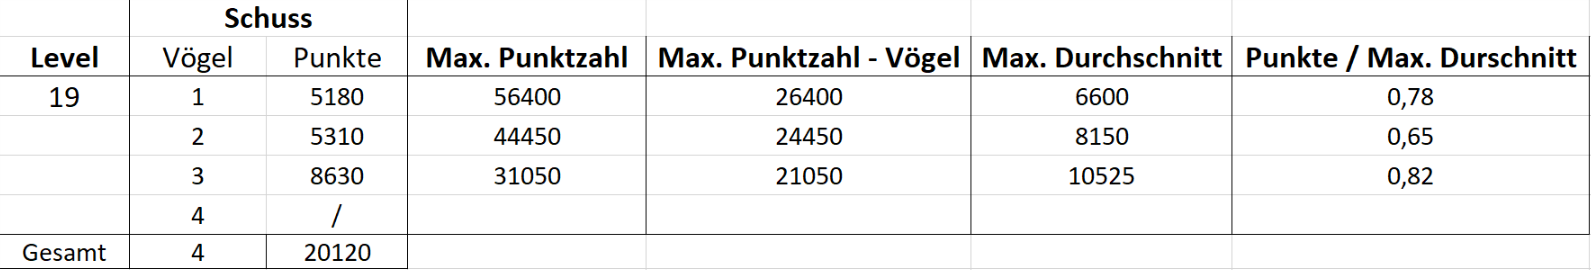
\includegraphics[width=1\textwidth]{Level19}
   \caption{Level 19}
   \label{lvl19}
\end{figure}


Grund für Limit, beispielsszenario


\subsection{Meta}
Das Zusammenspiel aller oben genannten Klassen findet in der \menu{ meta > Meta}-Klasse statt, welche von der Hauptinstanz \menu{ main > Bambird} aufgerufen wird. Diese Klasse stellt die Verbindung zum tatsächlichen Spiel und dem Server dar. \\
Ein Objekt der Klasse \texttt{Meta} wird genau einmal aufgerufen und entspricht der eigentlichen Main-Methode. Zur Veranschaulichung des Aufbaus dieser Klasse dient der Pseudocode \ref{meta}.

\begin{algorithm}[H]
  \begin{algorithmic}[1]
  \If{shotCandidate.equals(previousShot)}
  \EndIf
  \end{algorithmic}
  \caption{Meta \label{meta}}
\end{algorithm}